% MASTER 8 -- Multilayer capacitance stack (simplified cross-section of Fig 2(b)). Covers Q11.
% Each layer forms an area capacitance to the substrate; add them in units of squareCg using
% C[squareCg] = (relative value) * area / (4 lambda^2).
%   metal   -> 0.075      poly -> 0.1      gate-to-channel -> 1
% Worked total in the notes: C_T = C_MS + C_PS + C_gC ~ 7.2 squareCg.
\documentclass[border=10pt]{standalone}
\usepackage{amsmath,amssymb}
\usepackage{tikz}
\usetikzlibrary{arrows.meta}
\begin{document}
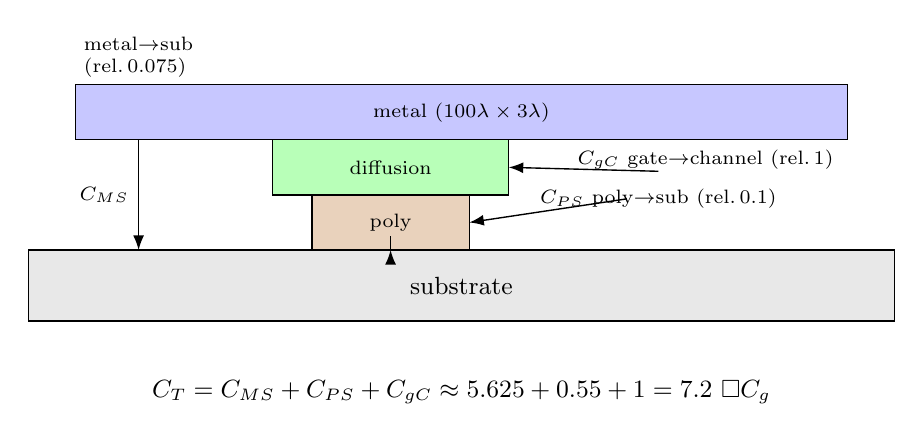
\begin{tikzpicture}[>=Latex,font=\small,line width=0.5pt]
% substrate
\fill[gray!18] (0,0) rectangle (11,0.9);
\node at (5.5,0.45) {substrate};
% polysilicon (small, bottom layer of the stack)
\fill[brown!35] (3.6,0.9) rectangle (5.6,1.6);
\node at (4.6,1.25) {\scriptsize poly};
% diffusion (middle)
\fill[green!28] (3.1,1.6) rectangle (6.1,2.3);
\node at (4.6,1.95) {\scriptsize diffusion};
% metal (long, top)
\fill[blue!22] (0.6,2.3) rectangle (10.4,3.0);
\node at (5.5,2.65) {\scriptsize metal  ($100\lambda\times3\lambda$)};
% outlines
\draw (0,0) rectangle (11,0.9);
\draw (3.6,0.9) rectangle (5.6,1.6);
\draw (3.1,1.6) rectangle (6.1,2.3);
\draw (0.6,2.3) rectangle (10.4,3.0);
% capacitance call-outs to substrate
\draw[->] (1.4,2.3) -- (1.4,0.9) node[midway,left,font=\scriptsize]{$C_{MS}$};
\node[font=\scriptsize,align=left] at (1.4,3.35) {metal$\to$sub\\(rel.\,0.075)};
\draw[->] (4.6,0.9) -- (4.6,0.9);  % poly sits on substrate edge
\node[font=\scriptsize,align=center] at (8.0,1.55) {$C_{PS}$ poly$\to$sub (rel.\,0.1)};
\draw[->] (7.6,1.55) -- (5.6,1.25);
\node[font=\scriptsize,align=center] at (8.6,2.05) {$C_{gC}$ gate$\to$channel (rel.\,1)};
\draw[->] (8.0,1.9) -- (6.1,1.95);
% total
\node[align=center] at (5.5,-0.9)
  {$C_T=C_{MS}+C_{PS}+C_{gC}\approx 5.625+0.55+1=7.2\ \square C_g$};
\end{tikzpicture}
\end{document}
